\documentclass[12pt]{article}

\usepackage{enumerate}
\usepackage{graphicx}
\usepackage{geometry}
\usepackage{float}
\usepackage{appendix}
\usepackage{color}
\usepackage{amsmath}
\usepackage{pifont}
\usepackage{fancyhdr}
\usepackage{enumitem}
\usepackage{amssymb}
\usepackage{cite}
\usepackage{url}
\fancyhf{}


\geometry{a4paper}
\geometry{left = 2cm}
\geometry{right = 2cm}
\geometry{top = 3cm}
\geometry{bottom = 3cm}

\pagestyle{fancy}
\lhead{STA130H1}
\rhead{Project Final Report}
\cfoot{\thepage}

\title{STA130H1 Capstone Project Final Report}

\author{Xuanqi Wei, Shujun Yang, Riyad Valiyev, Nicolas Dias Martins}

\date{\today}

\begin{document}


\maketitle
\thispagestyle{empty}

\newpage

\tableofcontents
\thispagestyle{empty}

\newpage

\setcounter{page}{1}

\section{Abstract}
The present investigation is rooted in a fundamental curiosity to deepen our understanding of the cosmos in which we reside and to shed light on the enigmas that surround celestial objects and their properties. By approaching our research questions from a statistical perspective, we aspire to uncover novel associations between various attributes of galaxies and to account for their interrelationships. To achieve these objectives, we employ a range of statistical tools and techniques, including bootstrapping, constructing confidence intervals, hypothesis testing, and linear regression.

\noindent
Our findings reveal a significant correlation between brightness and redshift, indicating that galaxies that are farthest from Earth differ markedly from their closer counterparts in terms of total luminosity. Furthermore, we have observed that the total size of a galaxy may be linked to the proportion of light contained within its radius. In order to ensure the validity and reliability of our results, we have employed hypothesis tests to evaluate the robustness of our findings.

\noindent
The results of this study offer insight into the complex relationships that exist among stars and galaxies and provide a foundation of knowledge that can be applied to further exploration and investigation in this field. Ultimately, our aim is to enhance our comprehension of the universe and contribute to the advancement of astronomical research.

\newpage

\section{Research Question 1: How is the galaxy's total size related to the percentage of light within the radius?}

\subsection{Introduction}

There are three different variables in the NSA table (available in `Galaxy Zoo Tabular Data Contents') related to a galaxy's size (in radius): `petro\_th50', `petro\_theta', and `petro\_th90'. Based on the aforementioned variables, the goal of this research question is to answer how a galaxy's total size is related to the percentage of light within its radius.

\subsection{Data}

The data used in Research Question 1 comes from the NSA table \cite{NSA}, which includes multiple properties of galaxies. The properties analysed by this question are related to the variables `petro\_theta', which is an estimate of a galaxy's total size in radius, `petro\_th50', which is an estimate of a galaxy's size in radius where 50\% of the light is inside the radius and 50\% of the light is outside the radius, and `petro\_th90', which is an estimate of a galaxy's size in radius where 90\% of the light is inside the radius and 10\% of the light is outside the radius. According to the aforementioned descriptions, the `galaxy's total size' is related to the variable `petro\_theta', while the `percentage of light within the radius' is related to variables `petro\_th50' and `petro\_th90'. In addition to that, the data was cleaned, removing any NA and extreme values (outliers) for all variables in the NSA table.

\subsection{Method \& Analysis}

The method used in Research Question 1 is bootsprapping and confidence intervals. Bootstrapping is a process used to simulate a sampling distribution of a specific sample statistics by random sampling with replacement, while confidence intervals 

\noindent
Firstly, the data was cleaned, removing any NA and extreme values (outliers) for all variables in the NSA table. In order to remove the outliers, it was necessary to find the Interquantile Range (IQR) for each variable analysed (`petro\_th50', `petro\_theta', and `petro\_th90') and remove all values above an upper limit and below a lower limit, which are both defined by the IQR. By the end of this process, 82,089 observations were removed from the original data table.

\noindent
After cleaning the data, three bootstrap histograms were built based on the means of each variable analysed. In order to plot those, it was necessary to run 1000 bootstrap simulations (with replacement) using the full cleaned data containing 559,320 observations as the sample. Afterwards, 90\% confidence intervals were computed for the bootstrap means for each variable analysed.  

\subsection{Results}

By describing the methodology described above, we got three diferrent bootstrap distribution graphs (which is a plot that shows the distribution of a  statistics boot sample):

\begin{enumerate}
	\item The first bootstrap sampling distribution graph (graph 1) is related to the mean values of the `petro\_th50' statistic from the boot samples. The x-axis is the range of possible mean values of `petro\_th50' from the boot samples, while the y-axis is the frequency (count) of a specific mean value. All mean values of `petro\_th50' are around 2.61 - 2.62.
	\item The second bootstrap sampling distribution graph (graph 2) is related to the mean values of the `petro\_theta' statistic from the boot samples. The x-axis is the range of possible mean values of `petro\_theta' from the boot samples, while the y-axis is the frequency (count) of a specific mean value. All mean values of `petro\_theta' are around 5.68 - 5.70.
	\item The third and last bootstrap sampling distribution graph (graph 3) is related to the mean values of the `petro\_th90' statistic from the boot samples. The x-axis is the range of possible mean values of `petro\_th90' from the boot samples, while the y-axis is the frequency (count) of a specific mean value. All mean values of `petro\_th90' are around 6.88 - 6.90.
\end{enumerate}
\noindent
After that, by computing the confidence intervals for each variable analysed, we got to the following results:
\begin{enumerate}
	\item We are 90\% confident that the mean value of the galaxy's size in radius (where 50\% of the light is inside the radius and 50\% of the light is outside the radius) for all universes in the NSA table is between 2.616138 and 2.620720 (image 1).
	\item We are 90\% confident that the mean value of the galaxy's total size in radius for all universes in the NSA table is between 5.682789 and 5.692060 (image 2).
	\item We are 90\% confident that the mean value of the galaxy's size in radius (where 90\% of the light is inside the radius and 90\% of the light is outside the radius) for all universes in the NSA table is between 2.616138 and 2.620720 (image 3).
\end{enumerate}
Based on everything we got from our methodology, it is possible to infer that a galaxy's total size may be related to the percentage of light within its radius, as the mean of the total size (petro\_theta) of the set of galaxies analysed is always between the mean of 'petr\_th50' (galaxy's size in radius where 50\% of the light is inside the radius and 50\% of the light is outside the radius) and petro\_th90 (galaxy's size in radius where 90\% of the light is inside the radius and 90\% of the light is outside the radius) for the set of galaxies analysed.
\newpage

\subsection{Data Visulization}

\begin{figure*}[h]
	\centering
	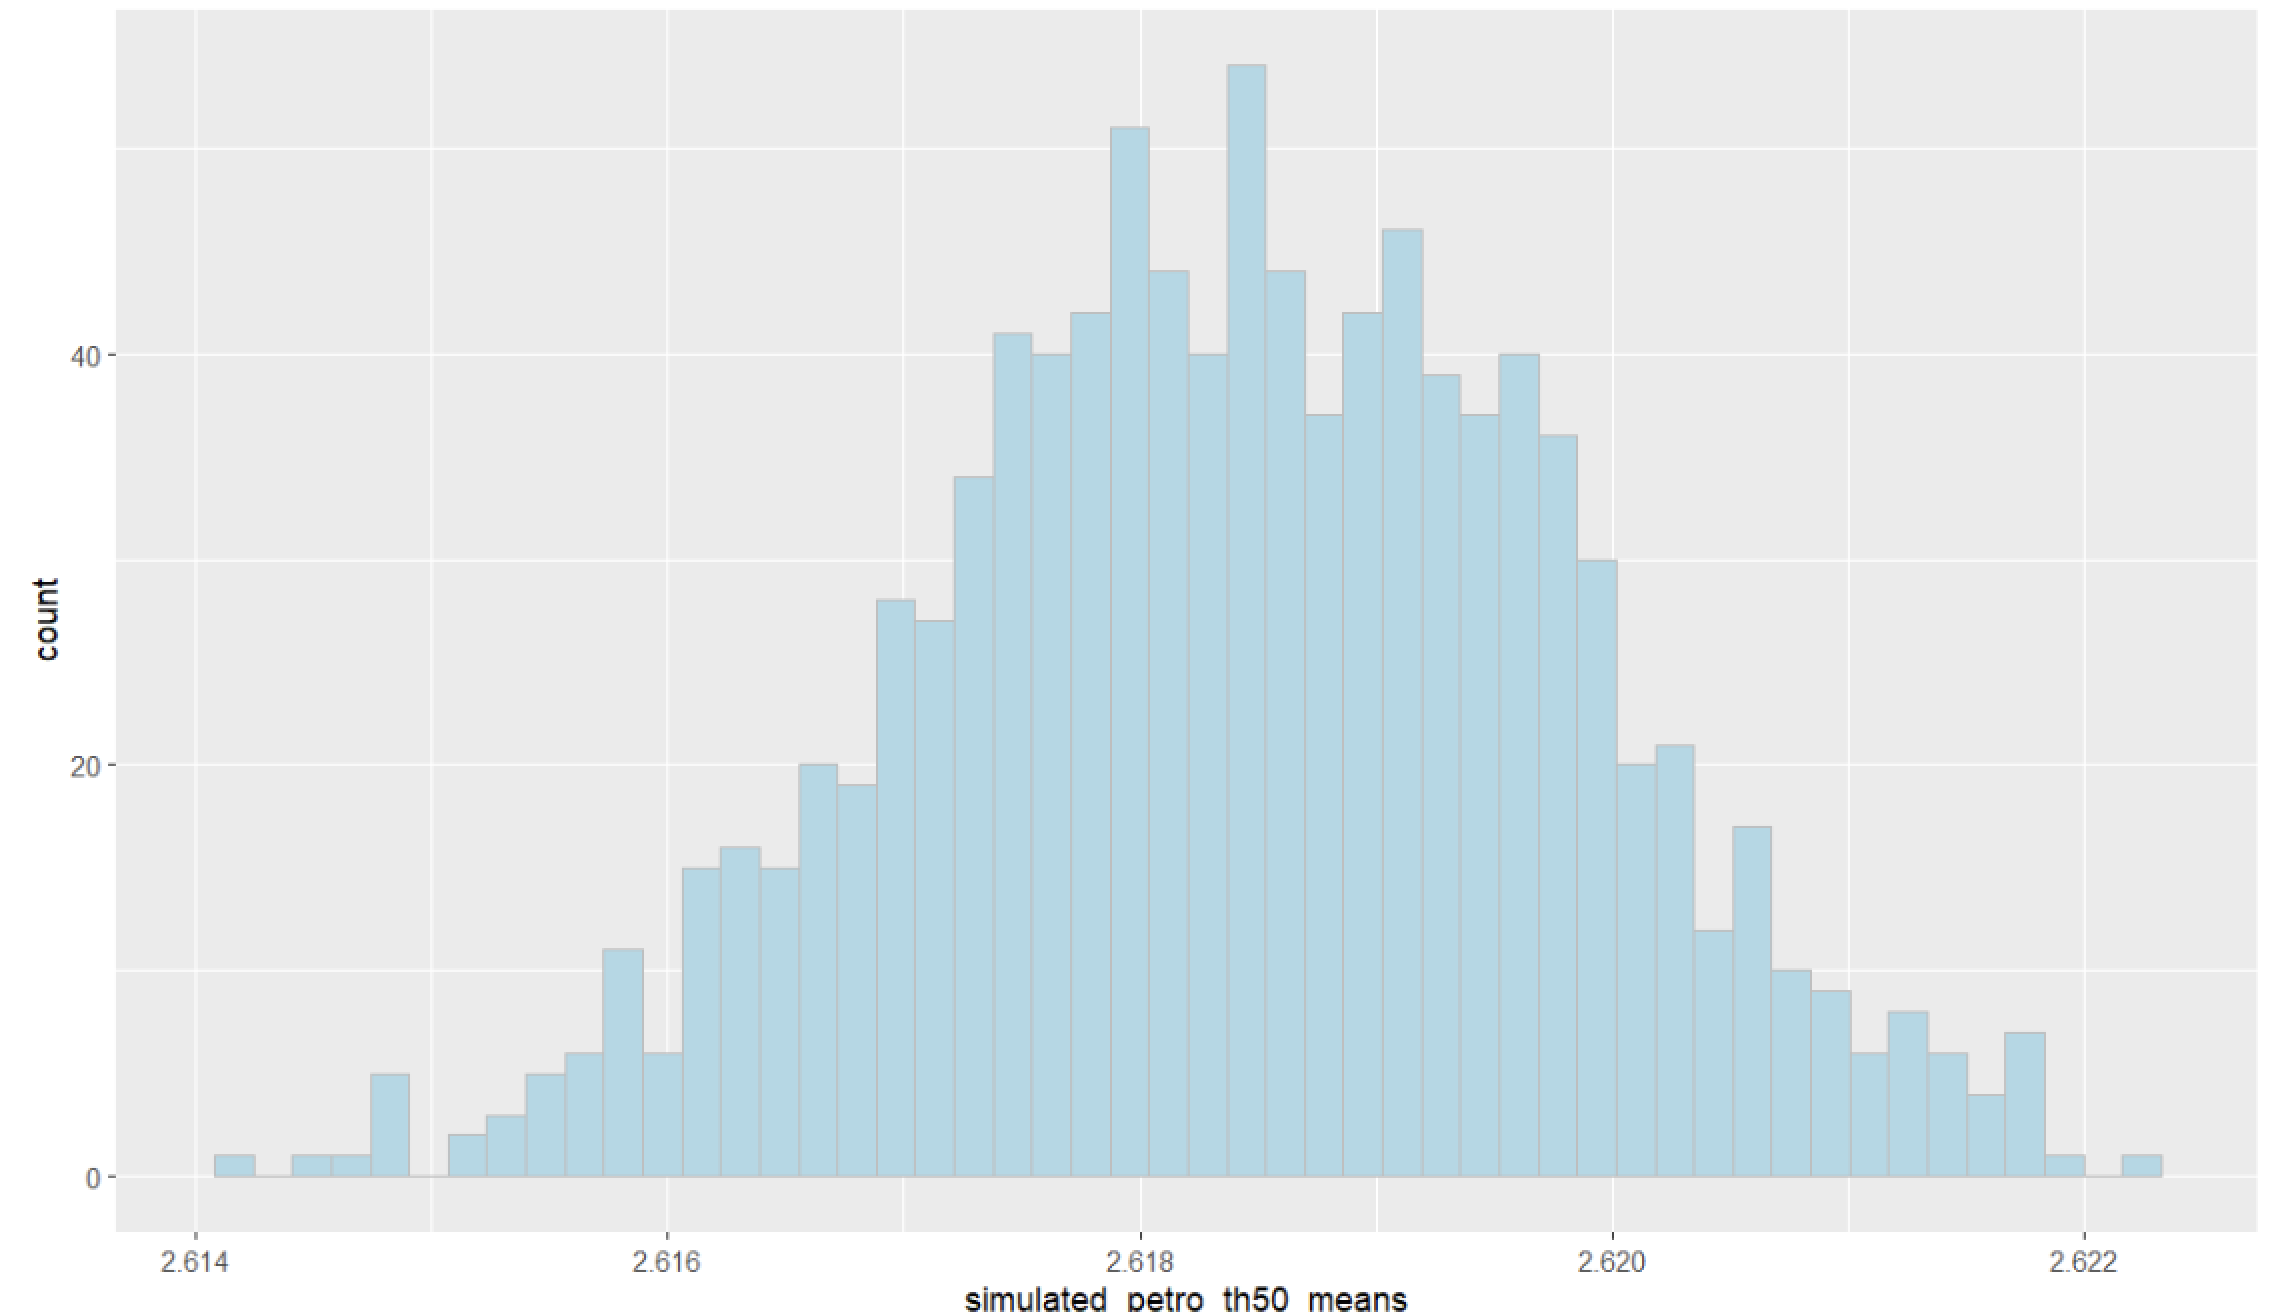
\includegraphics[width=0.6\textwidth]{pic/50_h.png}
	\caption{Bootstrap histogram of the mean of petro\_th50}
\end{figure*}

\begin{figure*}[h]
	\centering
	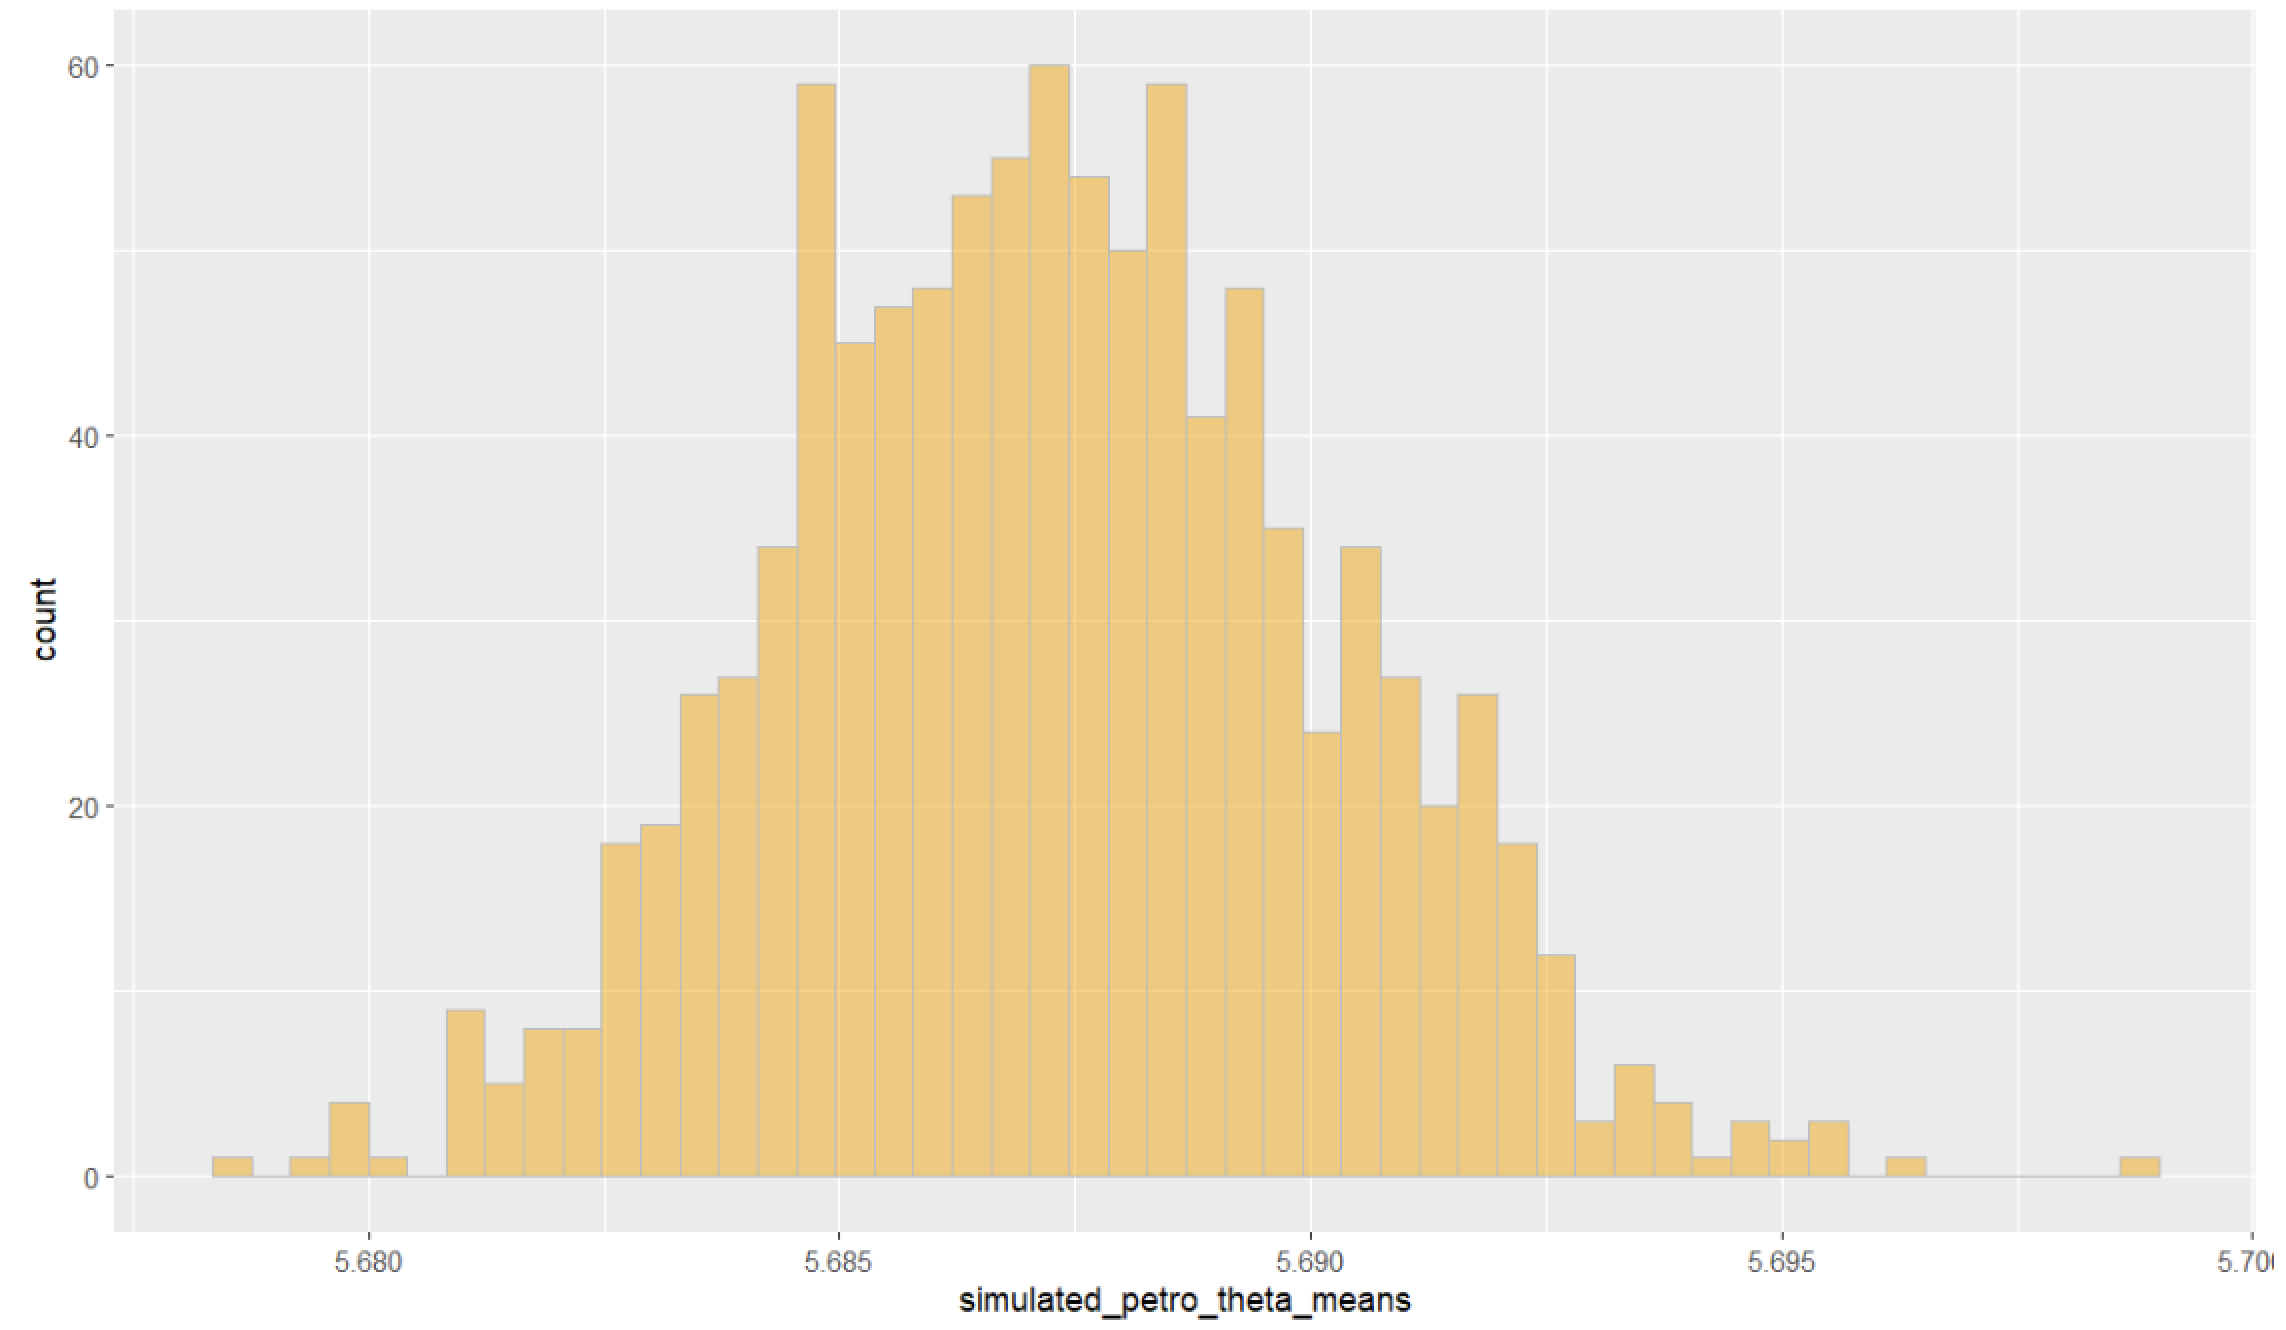
\includegraphics[width=0.6\textwidth]{pic/the_h.png}
	\caption{Bootstrap histogram of the mean of petro\_theta}
\end{figure*}

\begin{figure*}[!h]
	\centering
	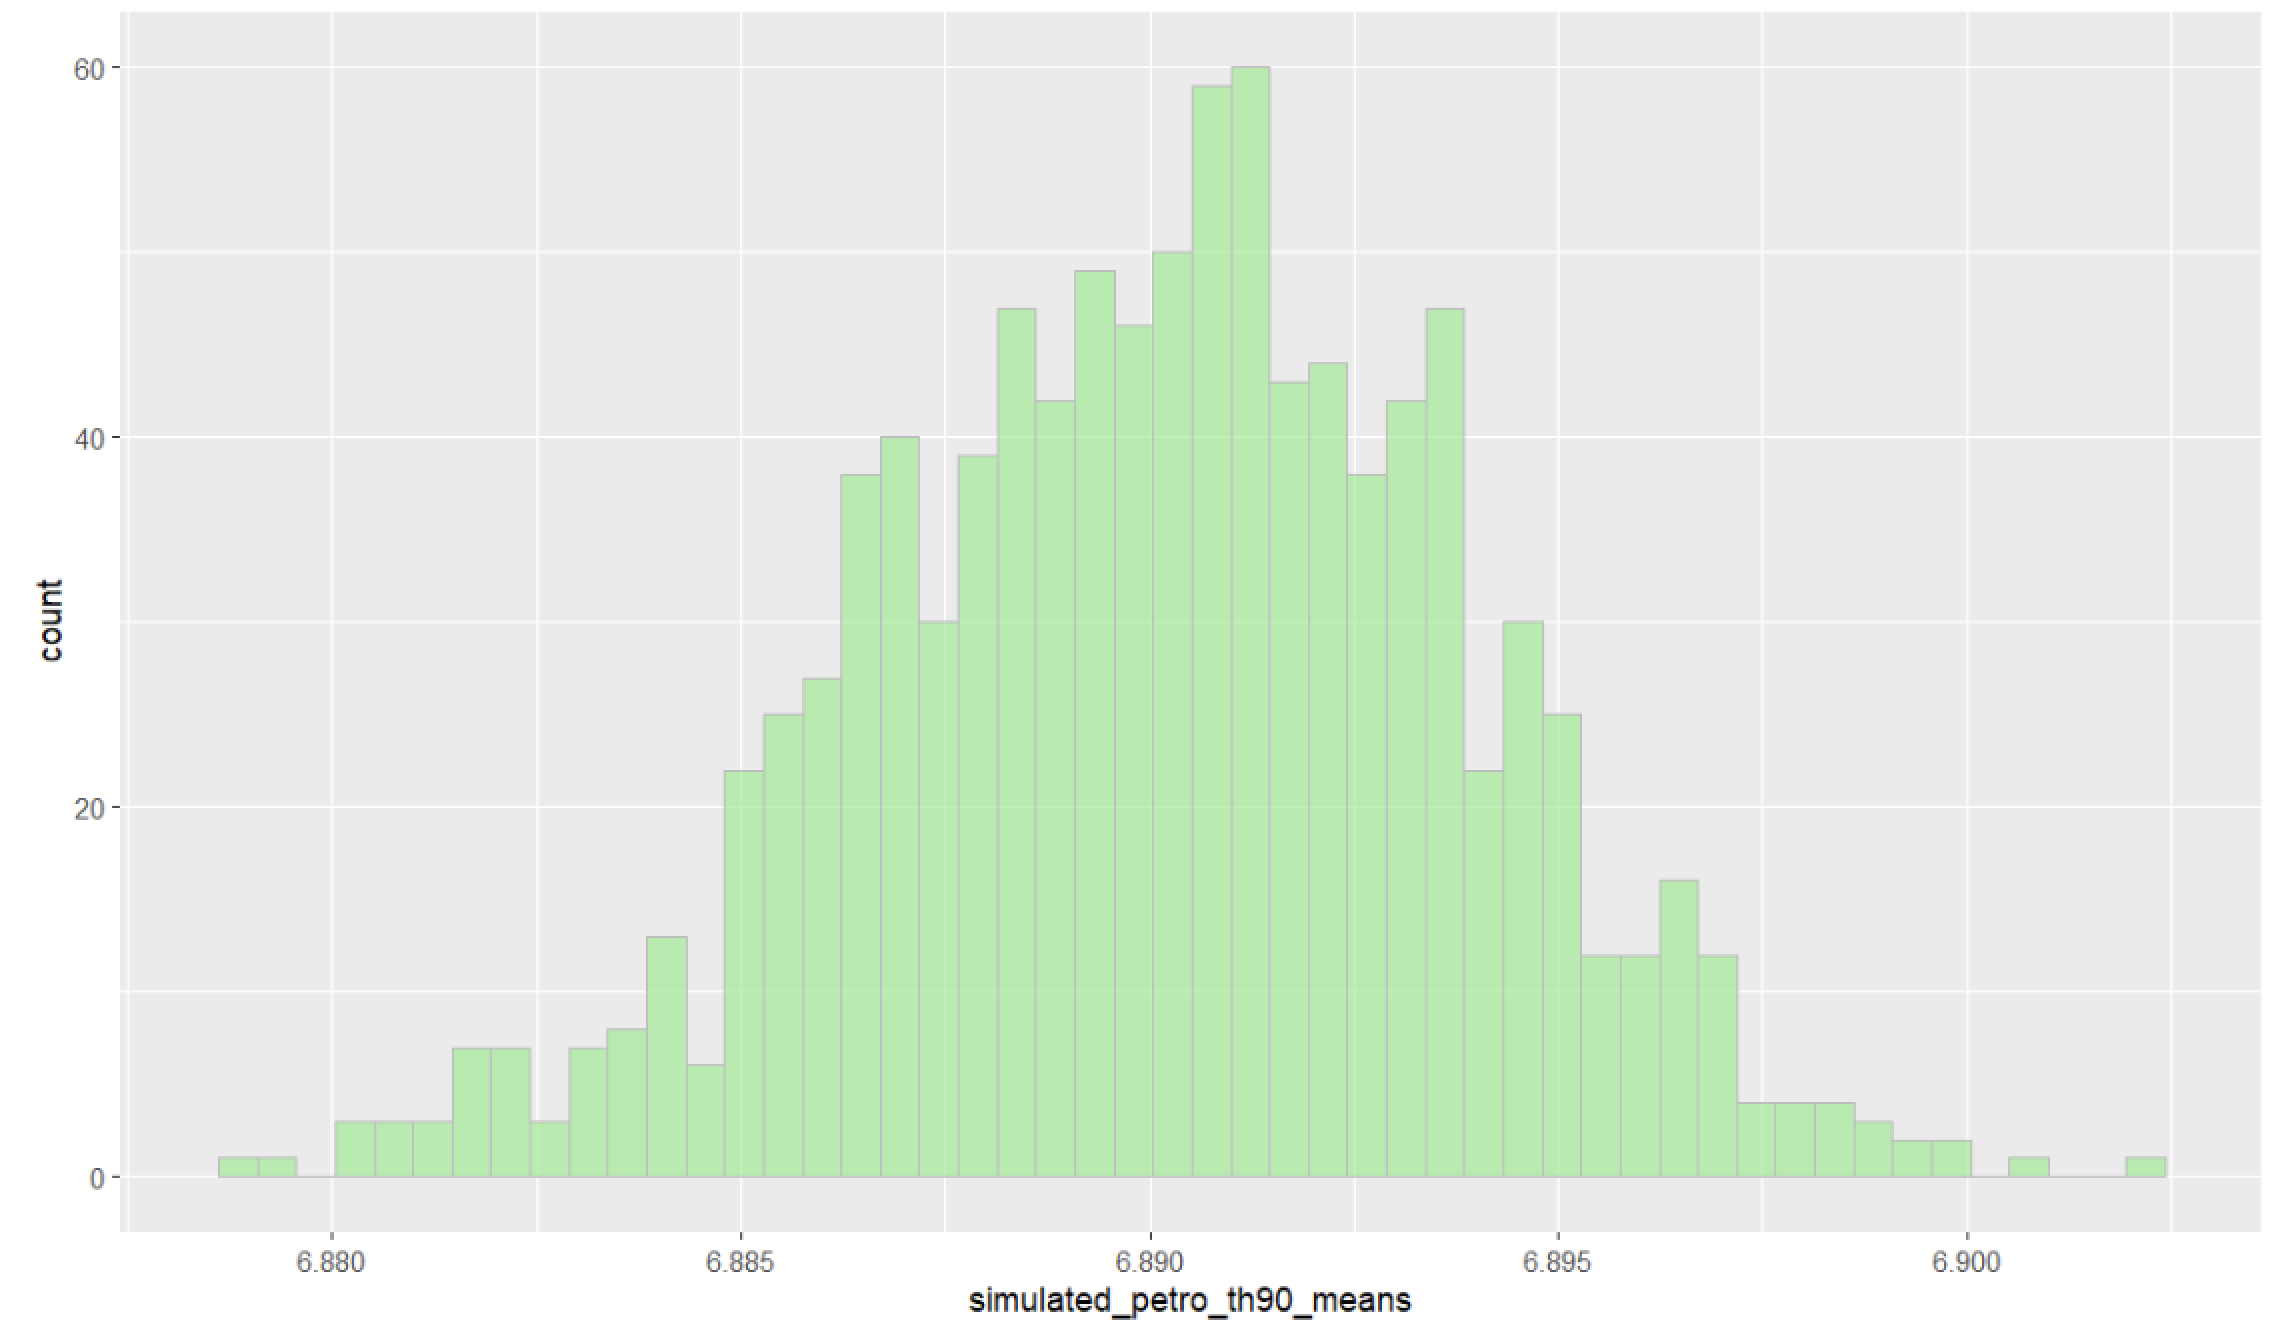
\includegraphics[width=0.59\textwidth]{pic/90_h.png}
	\caption{Bootstrap histogram of the mean of petro\_th90}
\end{figure*}


\begin{figure*}[h]
	\centering
	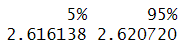
\includegraphics{pic/50_t.png}
	\caption{Confidence Interval (90\%) for petro\_th50}
\end{figure*}

\begin{figure*}[!h]
	\centering
	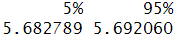
\includegraphics{pic/the_t.png}
	\caption{Confidence Interval (90\%) for petro\_theta}
\end{figure*}

\begin{figure*}[!h]
	\centering
	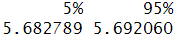
\includegraphics{pic/the_t.png}
	\caption{Confidence Interval (90\%) for petro\_90}
\end{figure*}

\newpage
\subsection{Discussion}
Our analysis of the NSA table suggests that there is a relationship between the range of the three variables analysed, which are all related to a galaxy's size in different ways. This result has interesting implications on how a galaxy's total size may be measured and how it is related to the percentage of light within this galaxy radius. However, our results are not perfect and future research can check if the relationship between these variables is based on randomness or not (by doing hypothesis testing).


\subsection{Conclusion}
To conclude, the goal of Research Question 1 was to answer how a galaxy's total size is related to the percentage of light within its radius. In order to answer it, we used the data from the NSA table, which contains three relevant variables for the question, all related to a galaxy's size: `petro\_th50' (an estimate of a galaxy's size in radius where 50\% of the light is inside the radius and 50\% of the light is outside the radius), `petro\_theta' (galaxy's total size in radius), and `petro\_th90' (an estimate of a galaxy's size in radius where 50\% of the light is inside the radius and 50\% of the light is outside the radius). By doing the bootstrapping process with the mean value of these variables and afterwards getting the 90\% confidence intervals for the means of each variable, we could finally conclude that it is possible to infer that a galaxy's total size may be related to the pergentage of light within its radius, as the mean of the total size (petro\_theta) of the set of galaxies analysed is always between the mean of `petro\_th50' and `petro\_th90' for the set of galaxies analysed. 

\newpage

\section{Research Question 2: Do the galaxies farthest to the Earth differ significantly from the closest ones in terms of their total luminosity?}

\subsection{Introduction}

The driving motivation for the statistical analysis outlined below is our aspiration to find out some of the mysteries of our universe by exploring the relationships among the celestial objects that roam in it. The question that we have put forward to base our research on in this section is the following: "Do the galaxies farthest to the Earth differ significantly from the closest ones in terms of their total luminosity?". In the hopes of discovering a definitive answer to this question, we will analyse the relationship between two of the attributes of our observed galaxies: their "total luminosity/intrinsic brightness" and their "redshift values" which could be expressed in a less technical way as "how far the given galaxy is located from the planet Earth". It is recommended that, before diving into our analysis, our readers familiarize themselves with the notion of hypothesis test, and in particular p-value, test statistic, null/alternative hypotheses, mean, sampling, shuffling and similar statistical terms so as to understand our results to the fullest.

\subsection{Data}

The data that we have utilized and will be accounting for throughout our report, Galaxy Zoo Tabular Data Contents, is taken from NASA-Sloan Atlas (nsa\_v1\_0\_1\_key\_cols.parquet) which was provided by Mike Walmsley. The data set includes a broad range of information regarding 641,409 distinct galaxies such as their stellar mass, star formation rates, shapes, et cetera. Amongst ten columns this data set contains, our focus will be on `redshift' and `elpetro\_absmag\_r' throughout this analysis, the latter one standing for the galaxy's total intrinsic brightness. The first thing we did upon downloading the data was to omit the values that are missing from the table, i.e. NA values, so that we would only take into account the observations with complete information in respective columns. Making sure that we carry out this data cleaning process before moving on to the integral parts of our analysis- implementing the methods, is very important in terms of ensuring the accuracy and minimal twistedness in our findings. Additionally, in one of the stages of our analysis that is specified below, we temporarily removed the mean `elpetro\_absmag\_r' values that lay outside of the interquartile range, being lower than 25th and higher than 75th percentiles, for the purposes of refining one of our visualization and delivering a clearer picture of the plot. Finally, one of the most critical steps we have taken in the entire research process was extracting two smaller subsets of the full data set: 1000 observations with the highest redshift values (corresponding to the galaxies in the data set that are farthest from the Earth) and 1000 observations with the lowest redshift values (corresponding to the galaxies in the data set that are closest to the Earth). We have saved these groups of observations in two distinct data frames and passed in just three variables for each: `redshift', `total intrinsic brightness', and a column indicating whether they belong to the `farthest' or `closest' category of galaxies.

\newpage
\begin{figure*}[h]
	\centering
	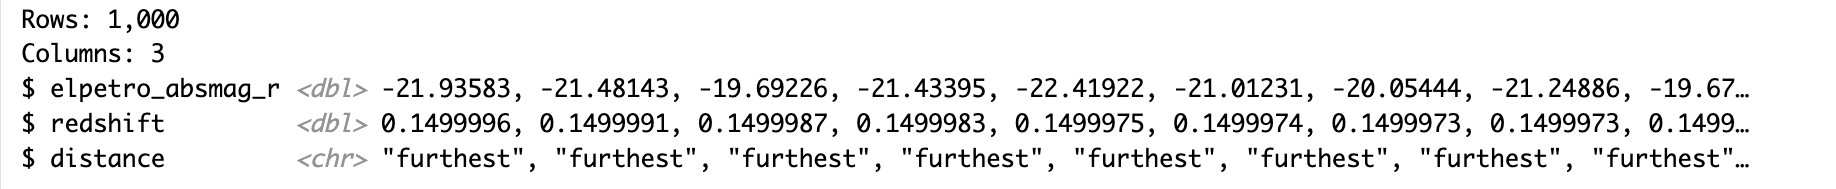
\includegraphics[width=1.0\textwidth]{pic/r2t0.png}
	\caption{Furthest}
\end{figure*}

\begin{figure*}[h]
	\centering
	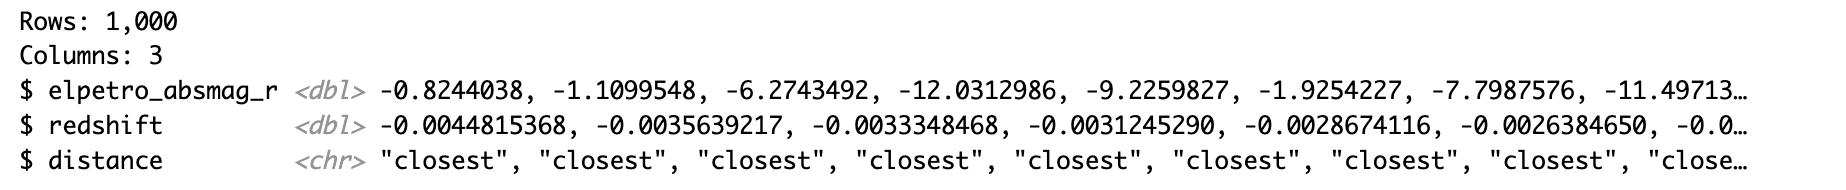
\includegraphics[width=1.0\textwidth]{pic/r2t1.png}
	\caption{Closest}
\end{figure*}


\subsection{Method \& Analysis}

On the way to addressing our main research question, we will making use of hypothesis test. In the first place, we will compute the absolute difference of the mean total luminosity values of these two groups (the furthest 1000 galaxies and closest 1000 ones). The result we'll get from this computation will give us some intuition towards the ultimate answer we seek. However, unless properly tested and verified, we can never be entirely sure if this result is just a product of some randomness that originates from the limitedness of our samples or is actually a significant finding. An at that point, hypothesis test will help us establish whether the difference (if any) indeed implies a general rule for the whole population of galaxies in the universe, or we cannot conclude such a general rule of "distance affecting brightness" simply because it could be a coincidence. The test will be ran under the null assumption that the aforementioned difference is zero, or put in another way, the mean luminosities of the groups are equal to each other. Our test will consist of 10,000 simulations where each simulation will involve shuffling 2,000 observations with "furthest" and "closest" attribute and assign them randomly to either category. Later, we will compute the p-value based on the percentage of the cases where we obtain at least as extreme difference as what we have measured, between the randomly shuffled groups.

\subsection{Results \& Data Visualization}

As the first step, we have analyzed the distribution of data in both groups through a number of numerical measures such as their minimum, maximum, mean, median values and standard deviation. Even though we are mainly interested in mean values of our sub-data sets, we took a quick look at median, range and standard deviation to have a rough understanding of what the shapes and skewness of our distributions look like and how much our mean values are impacted by the so-called "outlier bias". In particular, we intended to compare the median and mean values of each group to see how remote they are from each other (with the hopes that they would not be too much distanced). And in fact, our results at the first stage turned out to be quite promising for both categories:

\newpage

\begin{figure*}[h]
	\centering
	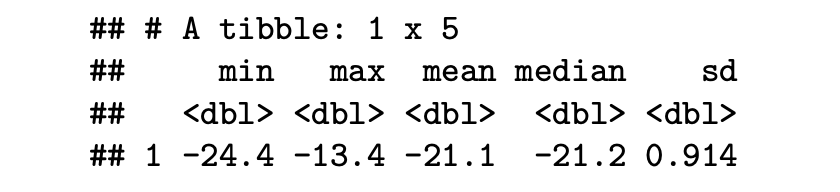
\includegraphics[width=0.55\textwidth]{pic/r2t2.png}
	\caption{Category 1}
\end{figure*}

\begin{figure*}[h]
	\centering
	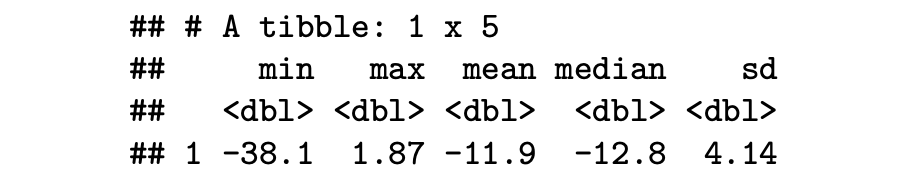
\includegraphics[width=0.6\textwidth]{pic/r2t3.png}
	\caption{Category 2}
\end{figure*}
\noindent
Later, we have plotted the mean values of these groups using a bar graph. In doing so, we wanted to visualize the comparison between the mean total brightness of "furthest" and "closest" galaxies, and make it more explicit through an illustration. While the mean total brightness of "closest" galaxies stood at around -12, that of the "furthest" ones was as low as around -21 absolute magnitudes. 

\begin{figure*}[h]
	\centering
	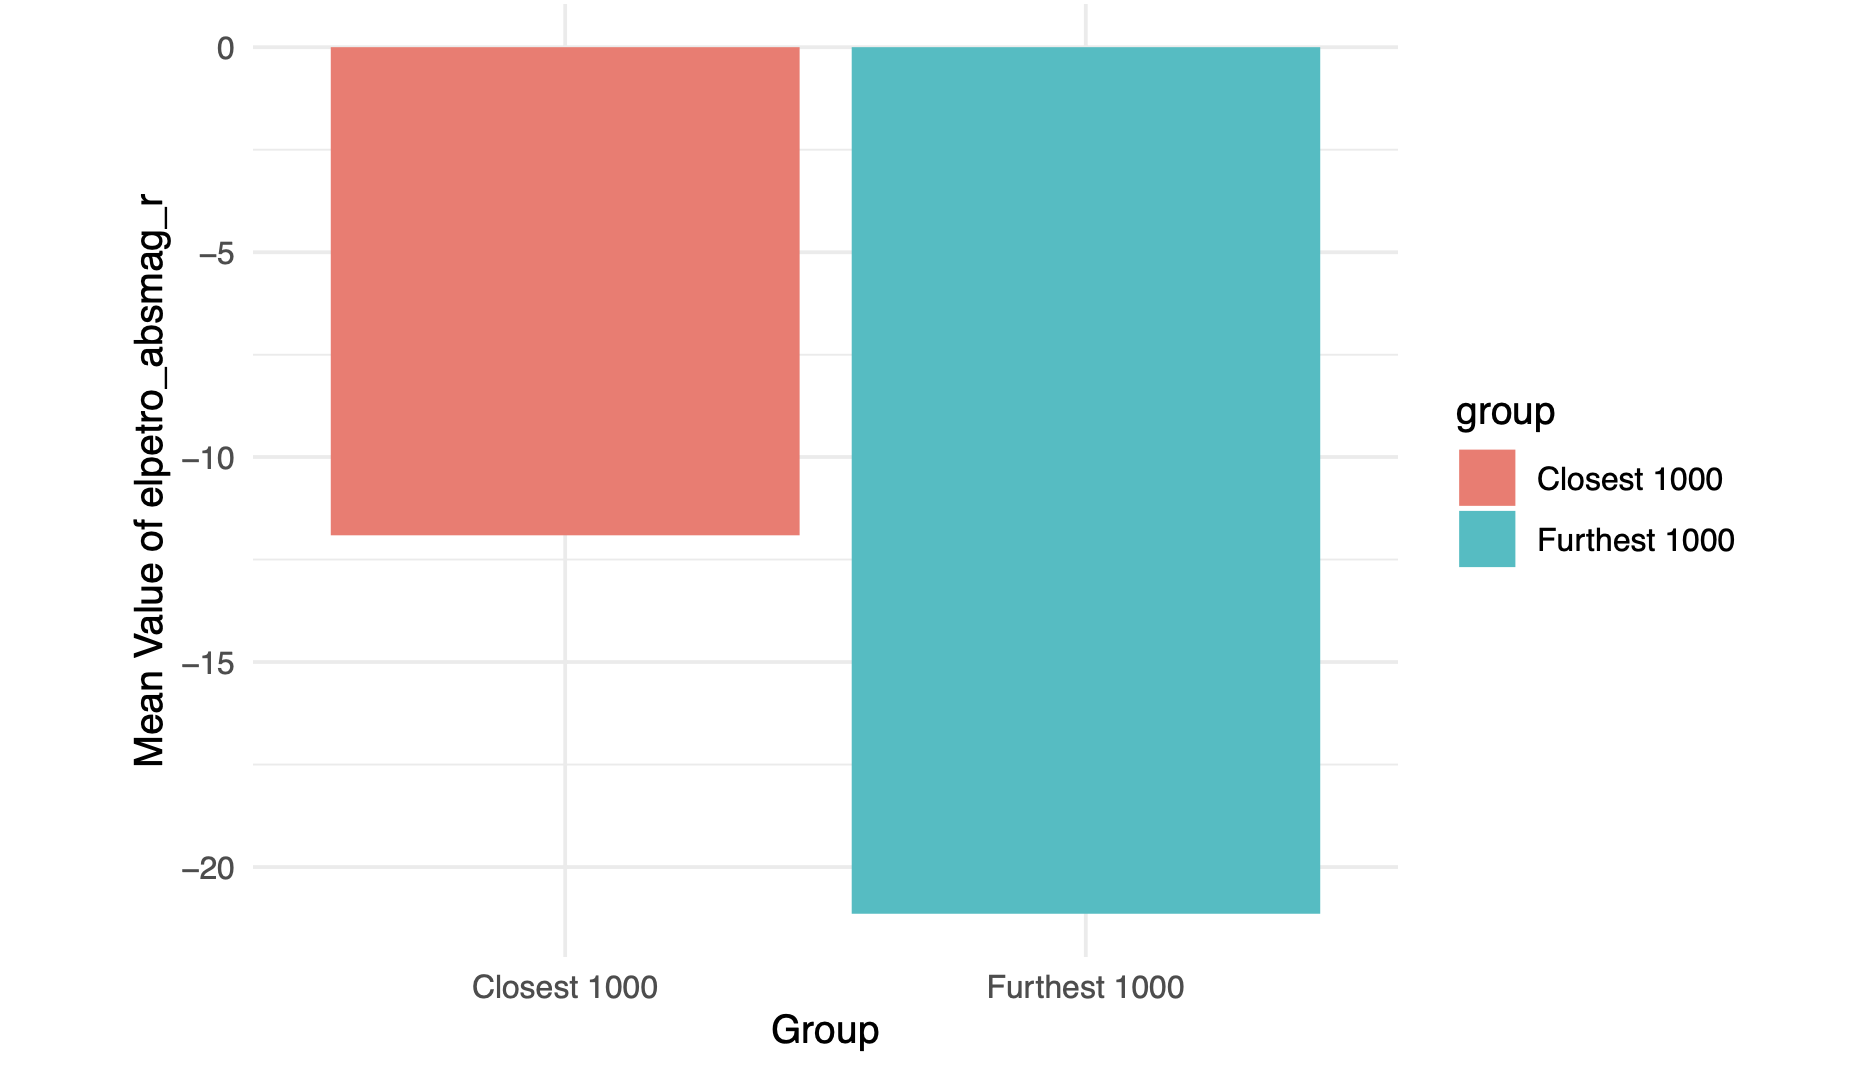
\includegraphics[width=0.9\textwidth]{pic/r2g1.png}
	\caption{Comparison of Mean Values}
\end{figure*}
\noindent
As we can see, the result is pretty noticeable. But we need to see if this is a part of some downward trend in the whole data set, suggesting a negative correlation between total brightness and redshift values, or just a random occurrence where the closest and furthest galaxies happened to have difference of 9 absolute magnitudes in terms of their mean total luminosities. To measure it, we grouped each 1000 rows of the data frame where ‘redshift’ is in an increasing order and got over 641 groups out of 641,166 observations. Next, we illustrated the line graph of the mean ‘elpetro absmag r’ values corresponding to each 1000-row group. The resulting line graph would need to have its x-axis correspond to each group of 1000 galaxies that are ordered as per their red-shift values (from least to most) and y-axis attributing to mean ‘elpetro absmag r’ of each group. One problem that we encountered while plotting this result was the outliers / unusually distant y-values. Given the sensitivity of line graphs to outliers, the extreme mean ‘elpetro absmag r’ values were distorting the shape of the graph, disfiguring the general trend and making it harder for the reader to follow the line. To tackle it, we removed the mean values that lay outside of the interquartile range (in other words, those higher than 75th percentile and lower than 25th percentile). Upon doing that, we got a more good-looking plot demonstrating an obvious downward tendency between the variables, and confirming our expectations:

\begin{figure*}[h]
	\centering
	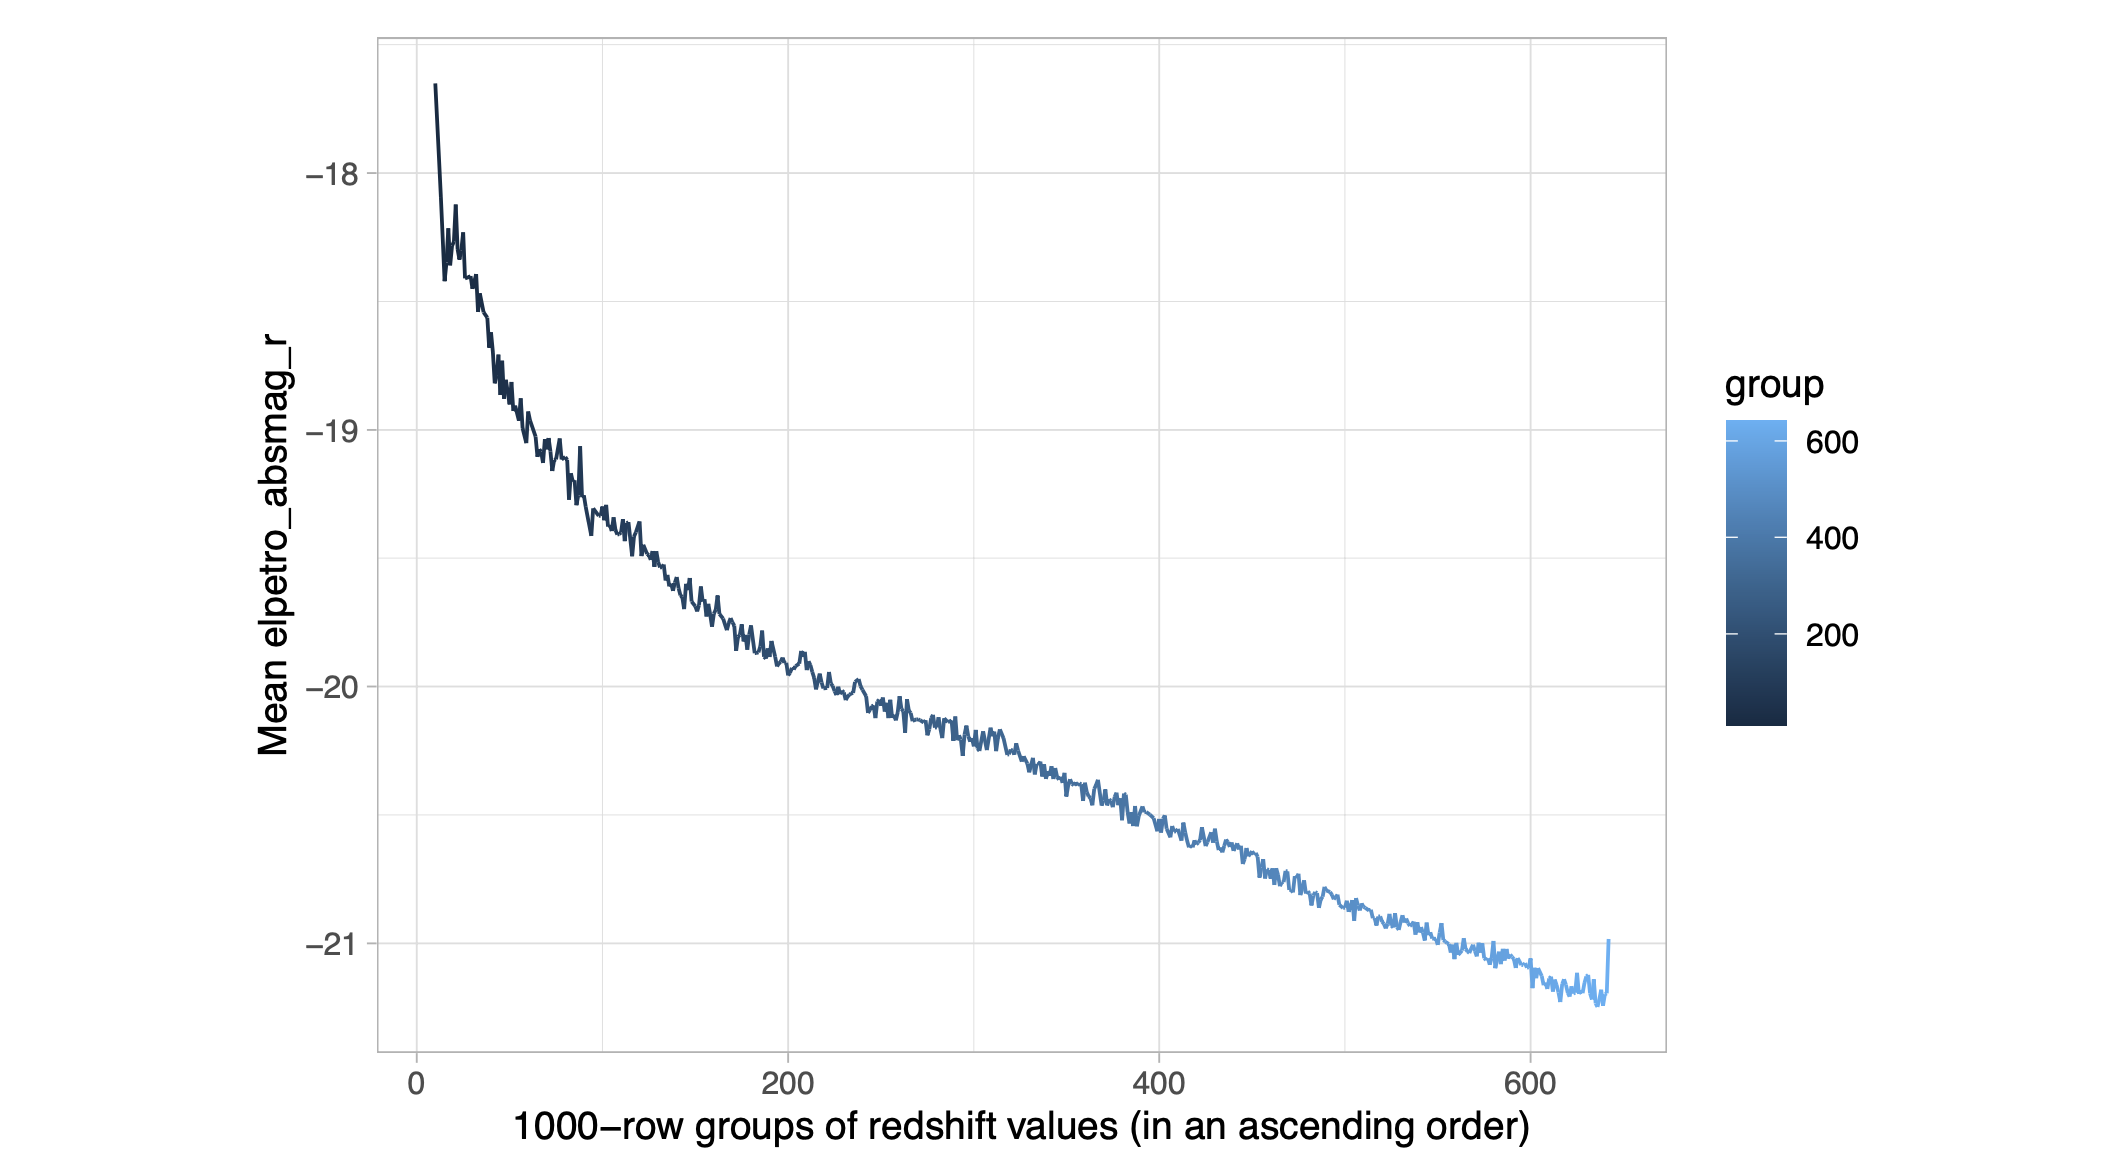
\includegraphics[width=0.9\textwidth]{pic/r2g2.png}
	\caption{Tendency}
\end{figure*}
\noindent
Next up, we have combined our two sub-data sets into a large one consisting of 2000 rows: 1000 from closest galaxies and 1000 from furthest ones. We have previously determined that the our test statistic (the actual difference between the mean total brightness of these groups) was around 9 absolute magnitudes. However, to make our calculations more precise, we calculated the test statistic anew using R computations and obtained the following:

\begin{figure*}[h]
	\centering
	
\includegraphics[width=1.0\textwidth]{pic/r2t4.png}
\end{figure*}
\noindent
Now that we have all of our tools at hand, we can run our 10,000 simulations and observe the results. As a reminder, our null hypothesis was that "there is no difference between the mean total luminosity of the farthest and closest galaxies" while the alternative hypothesis was stating exactly the opposite: "there is a difference between the mean total luminosity of the farthest and closest galaxies". Through the methods we have explained in the analysis section above, we will first plot the distribution of the 10,000 simulated values (that is, the difference between the mean total brightness of randomly shuffled groups) under the assumption that the null hypothesis is true:

\begin{figure*}[h]
	\centering
	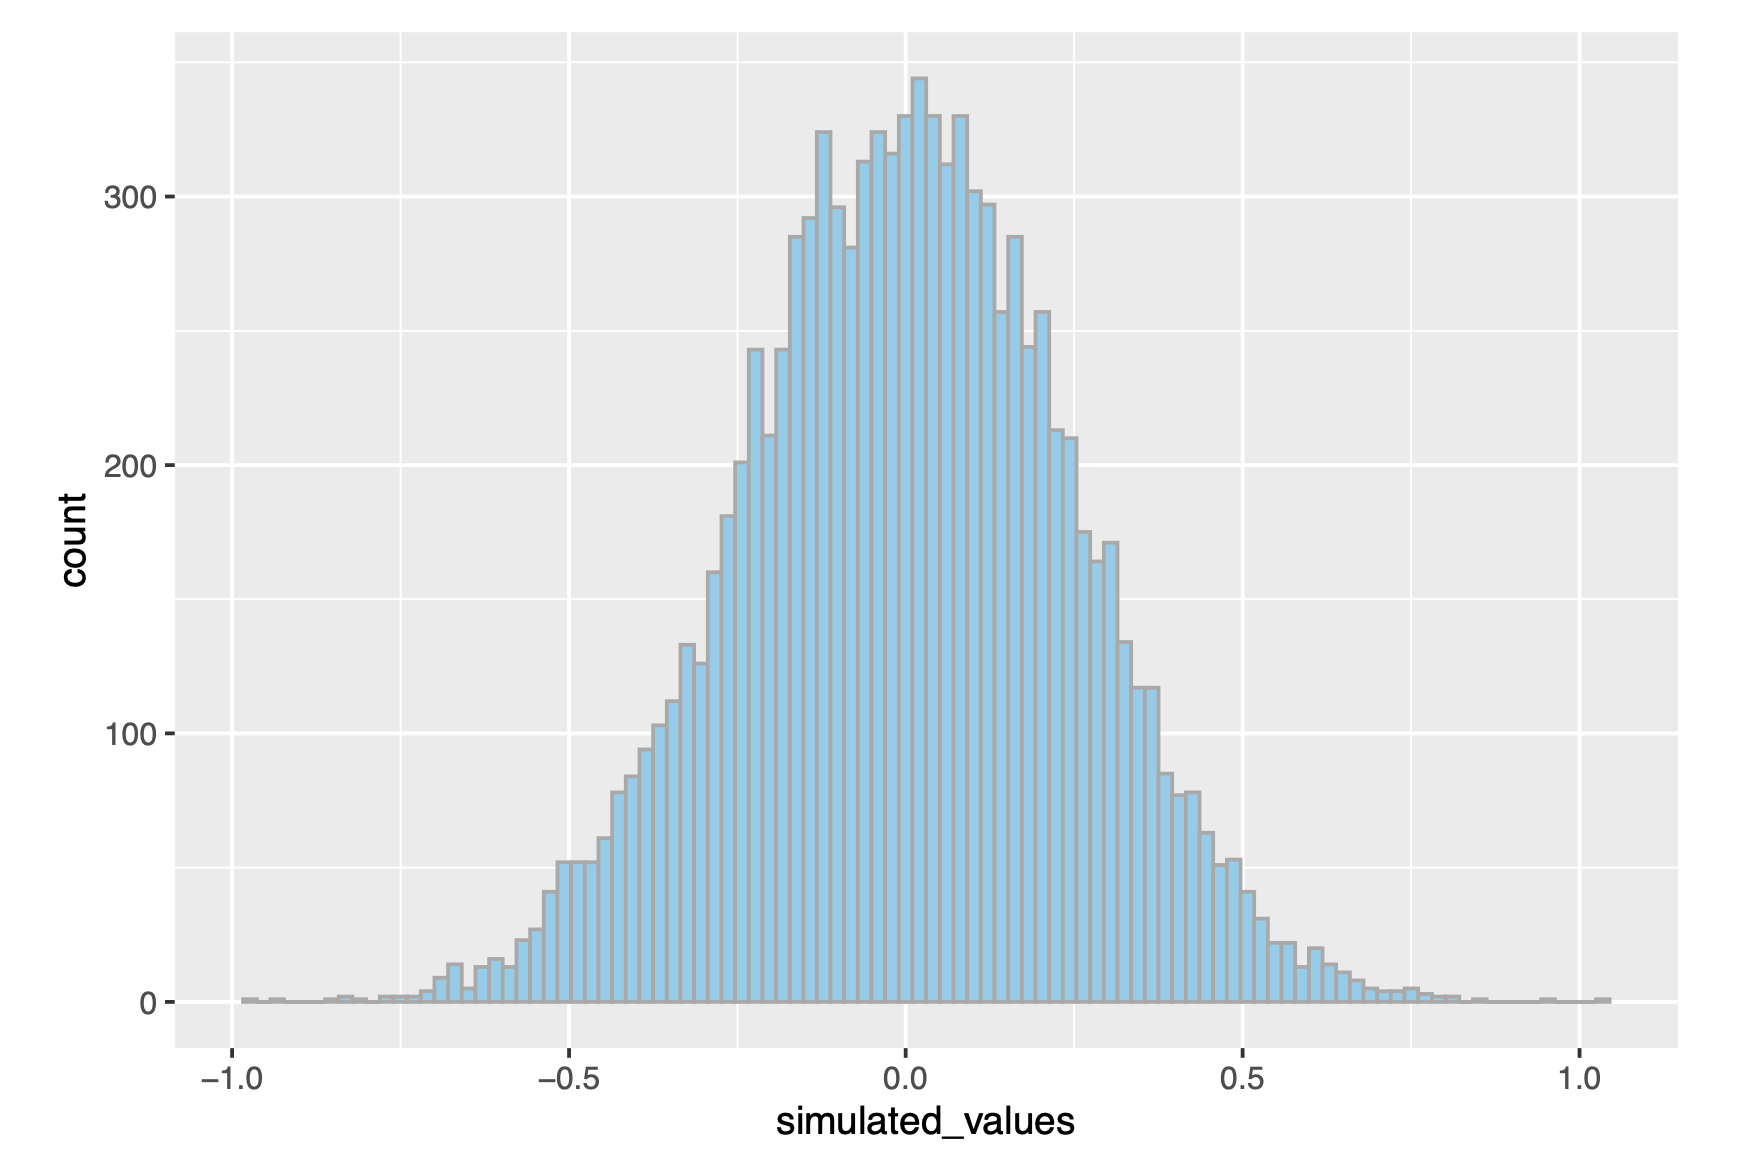
\includegraphics[width=0.9\textwidth]{pic/r2g3.png}
	\caption{Tendency}
\end{figure*}
\noindent
The results are pretty significant: we see a very large portion of the values gathered in an interval centered at 0.0. Which is even more significant, however, is the fact that the range of this interval is just around -1.0 and 1.0 (roughly). This preliminary observation, along with a quick glance at the histogram of this distribution, imply that there is almost no chance that a measurable amount of data would lie outside of the interval from -9.2 to 9.2. That being said, we made our final move and statistically approved our observations via numbers by computing the p-value. And we got the following:
\begin{figure*}[h]
	\centering
	
\includegraphics[width=1.0\textwidth]{pic/r2t5.png}
\end{figure*}
\noindent
In 0\% of the cases, the difference between the simulated groups was more than or equal to $|9.2|$, which is equivalent to saying the following statement: The probability that our measured difference of 9.2 could be due to randomness is 0!

\subsection{Discussion}

The fact that our computed p-value is 0 suggests that we don't even need a certain alpha level to be able to reject the null hypothesis. As our p-value falls under any possible alpha level $>$ 0 and successfully proves itself as being statistically significant in all cases, we can wholeheartedly assert that the idea that the furthest and closest galaxies might in fact have the same total luminosity should be rejected. Thanks to the hypothesis test, we discovered a correlation between two independent attributes of galaxies in the universe; what's more, our test helped us present this finding in such a way that an otherwise relationship could not be argued. 

\noindent
On top of it, we have also strengthened our findings by plotting the tendency between our variables that encompassed the entire data set. If our line graph visualizing the relationship of `elpetro\_absmag\_r' to increasing "redshift" values had had a `zigzag' pattern, there would have been a very good chance that our measured difference is due to randomness and does not account for any significant relationship. This would have also reflected itself in the p-value, as we would have most probably obtained a value way above 0. However, the fact that our line graph had a crystal-clear negative tendency all along the 641 groups of observations, was almost an announcement of the final results in advance of the time and something that filled us with a number of justifiable expectations.

\noindent
We have also showcased that the hypothesis test is an immensely powerful tool to utilize when we're in doubt of our results and pondering the question of `what if our findings just happened to turn out like this?'. Regardless of the magnitude of the measured results and how "significant" they appear to be, there is always a potential bias coming from the limitedness of the sample being worked on. Nonetheless, if one wants to generalize their findings achieved from `just a sample' to `the whole population', the hypothesis test is always a way to go!


\subsection{Conclusion}

To summarize, with an initial aim of discovering a relationship between the distances and total intrinsic brightness of the galaxies in the universe, we have firstly showed that there is a 9-unit difference between the mean total brightness of the furthest 1,000 and closest 1,000 galaxies with respect to the planet Earth in the data set. Using hypothesis test, we have revealed that this difference could not be achieved out of coincidence (if they were equal to each other) and acquired a 0 p-value in the process, proving that our measured findings were statistically significant. We have reinforced our point by constructing a line-graph that showcased an obvious downward trend between the variables that we were investigating.

\newpage

\section{Research Question 3: Do the galaxy's apparent brightness and the redshift linearly correlated?}

\subsection{Introduction}

In Galaxy Zoo Tabular Data content, there are two variables that might related which are `redshift' and `elpetro\_absmag\_r'. After draw their histogram, we find their shape is quite similar, they might have a relationship. Therefore we decide to investigate whether their is any relationship between brightness and the redshift .

\subsection{Data}
The data we used in research question 3 comes from `Galaxy Zoo Tabular Data Contents', more specifically, they're `redshift'\cite{redshift}, which is related to how far away that galaxy is from us, and, `elpetro\_absmag\_r', which is an estimate of the galaxy's total luminosity brightness or intrinsic brightness measured in absolute magnitude\cite{ab}.

\subsection{Method \& Analysis}

We did it in the following process:

\begin{enumerate}
	\item We update the data by loading libraries `tidyverse' and `arrow'\cite{CRAN}, and then remove the `NA' values.
	\item We use `ggplot' to get the histogram of both  `redshift'  and `elpetro\_absmag\_r', find that the histogram of redshift is unimodal approximately symmetric with a slight tendency towards the right side. The majority of the stars form this data set is between 0.07-0.075, which is in the middle of the range. The histogram of brightness is unimodal approximately symmetric with a slight tendency towards the left side. The majority of the stars form this data set is between -18.75 to -20, which is in the middle of the range. Both histogram have similar shape, it seems like they might have some relationship, but only analysis histogram can not tell that, we need to use linear regression model to see if the brightness and distance have a certain correlation.
	\item We create a linear regression plot, which `redshift' is the x-axis and ‘elpetro\_absmao\_r’ is the y-axis.
	\item We create a 'mod' the analysis the relationship between `redshif' and `elpetro\_absmag\_r. We apply `summary\$coefficients' to find the $\beta_1$, $\beta_0$ and p-value.The $\beta_0$ is the brightness when redshift equal to zero, which is -18.18. $\beta_1$ is the average change in brightness for 1 unit change in redshift which is - 22.75. Form here, we can get the linear regression model:
\begin{align*}
	y_i &= \beta_0 + \beta_1 x_i \\
	yi &= -18.18  - 22.75x_i 
\end{align*}

\end{enumerate}

\subsection{Results}
The p-value is 0 which is smaller than $\alpha$, we will reject $H_0$, support $H_1$. There is a linear relationship between brightness and redshift. Also the linear regression model: $y_i = -18.18 - 22.75x_i$ which shows a clear negative relationship between the brightness and redshift.

\noindent
It is important to note that although the p-value is significant and the linear relationship is strong, correlation does not necessarily imply causation. There may be other factors that contribute to the relationship between brightness and redshift, and further research may be needed to fully understand the underlying mechanisms.

\subsection{Data Visulization}

\begin{figure*}[h]
	\centering
	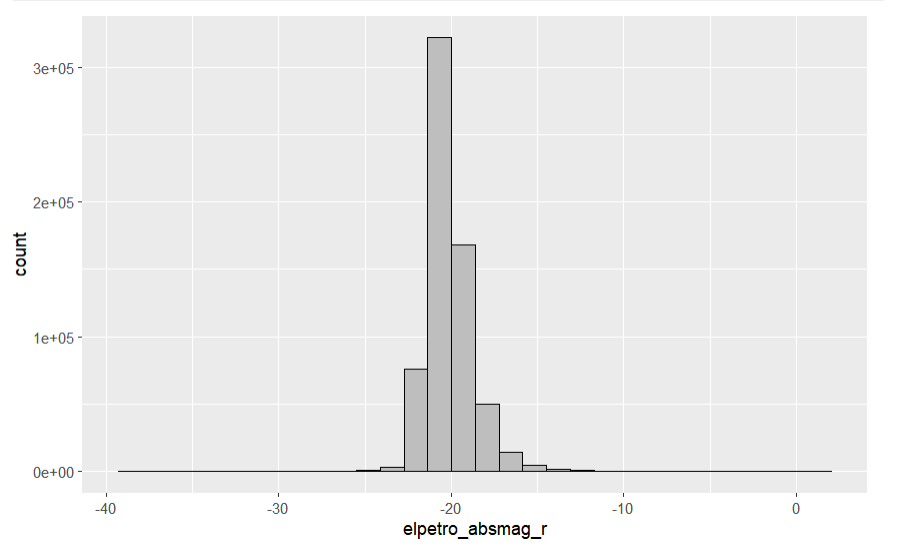
\includegraphics[width=0.7\textwidth]{pic/h1.png}
	\caption{Histogram of elpetro\_absmag\_r}
\end{figure*}

\begin{figure*}[h]
	\centering
	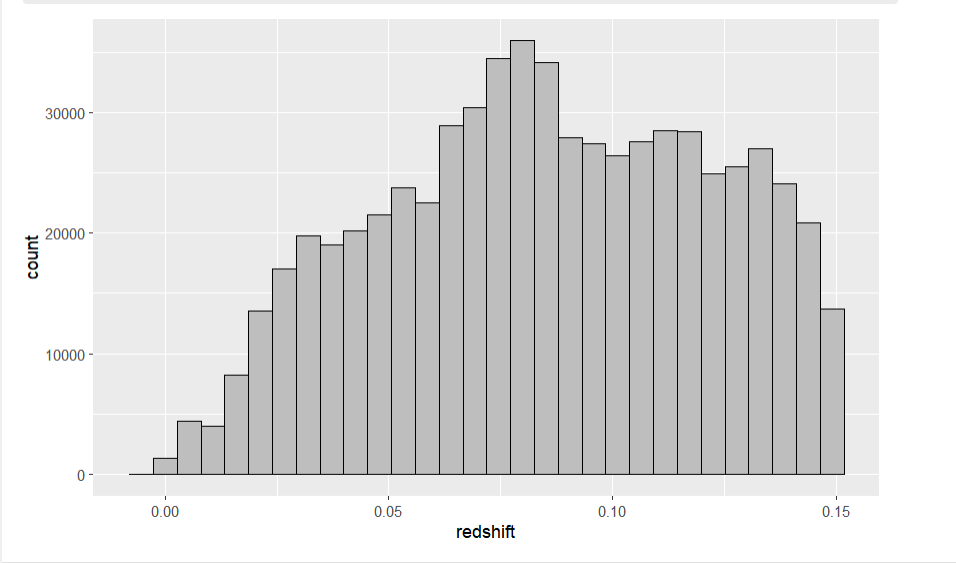
\includegraphics[width=0.7\textwidth]{pic/h2.png}
	\caption{Histogram of redshift}
\end{figure*}

\begin{figure*}[h]
	\centering
	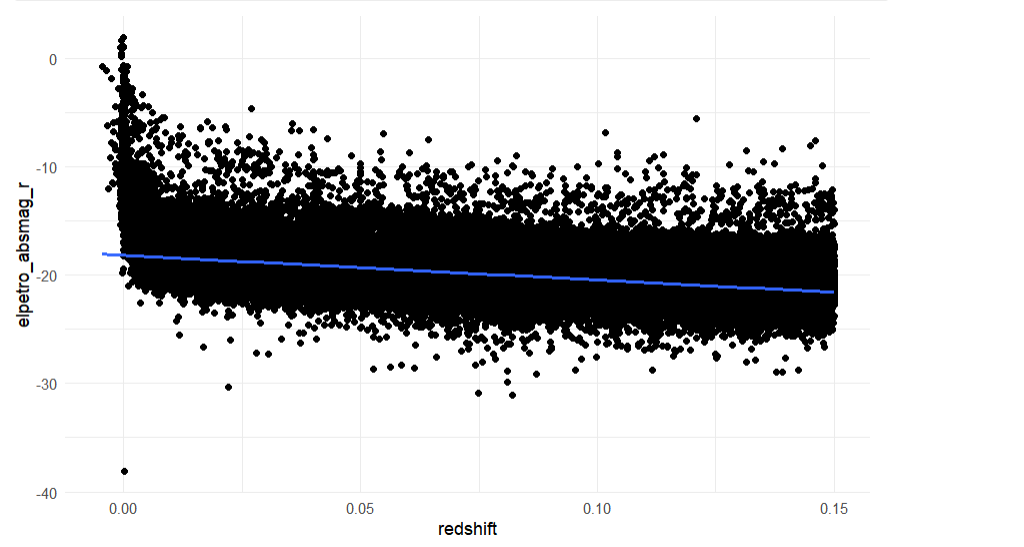
\includegraphics[width=0.8\textwidth]{pic/lr.png}
	\caption{Fitted Line Plot between redshift \& elpetro\_absmag\_r}
\end{figure*}



\newpage
\subsection{Discussion}

Our study of the Galaxy Zoo Tabular Data has yielded significant results indicating a strong linear correlation between the brightness and redshift of galaxies. This finding is consistent with our initial hypothesis and is supported by a p-value of 0, which indicates a high level of statistical significance. These results have important implications for our understanding of galactic properties, as they suggest that a galaxy's intrinsic brightness may be linked to its distance from Earth.

\noindent
However, it should be noted that further research is necessary to fully explore the nature of this relationship, as well as to identify other potential factors that may contribute to galaxy luminosity. Despite these limitations, our study provides a useful example of how statistical analysis can be leveraged to gain insights into complex and nuanced scientific phenomena.

\noindent
In conclusion, the results of our study underscore the importance of continued research into the properties of galaxies and their relationship to various external factors. By further exploring these relationships, we can deepen our understanding of the fundamental nature of the universe and the processes that shape it.

\subsection{Conclusion}
In summary, our study was based on a hypothesis regarding the relationship between redshift and brightness, which was suggested by comparing their histograms. We investigated this relationship using linear regression and ultimately confirmed a negative correlation between the two variables through a p-test. This finding provides insights and inspiration for our future work. If two datasets have similar histogram shapes, we can apply a linear regression model to obtain more accurate results.

\newpage

\section{Acknowledgement}

I would like to express my heartfelt gratitude to everyone who contributed to the successful completion of this capstone project. First and foremost, I would like to extend my sincere thanks to my friends, whose unwavering support and encouragement helped me stay motivated throughout the project. Their feedback and suggestions were invaluable in shaping the direction of my research and improving the overall quality of my work.

\noindent
I would also like to thank the teaching assistants who provided me with guidance and support throughout the course. Their patience and dedication in answering my questions and addressing my concerns were greatly appreciated, and played a crucial role in my understanding of the course material.

\noindent
Lastly, I would like to express my deepest appreciation to Professor Joshua Speagle, whose exceptional teaching and mentorship inspired me to pursue this project. His insightful feedback and constructive criticism challenged me to push my limits and strive for excellence, and I am grateful for the opportunity to learn from such a brilliant scholar.

\noindent
Overall, I am grateful to have had the support and guidance of such wonderful individuals throughout this capstone project, and I am confident that their contributions have played a significant role in its success.

\newpage

\bibliographystyle{plain}
\bibliography{ref}





\end{document}